\subsection{Vzájemná poloha parametricky vyjádřených přímek v prostoru}
\label{subsec:Relative_position_parametric_lines_space}

V rovině jsme zjistili, že dvě přímky mohou být různoběžné,
rovnoběžné nebo totožné. V prostoru se však objevuje ještě jedna
možnost. Dvě přímky mohou mít různé směry, a přesto se nemusí
protínat. Takové přímky nazýváme \textbf{mimoběžné}.

Uvažujme dvě přímky $p$ a $q$ zadané parametricky ve tvaru
\begin{align}
    p: X &= A+t\vec{u},
    \qquad t\in\mathbb{R},
    \label{eq:Parametric_line_p_relative_position_space}\\
    q: X &= B+s\vec{v},
    \qquad s\in\mathbb{R},
    \label{eq:Parametric_line_q_relative_position_space}
\end{align}
kde $A$ a $B$ jsou zvolené body jednotlivých přímek a
$\vec{u}$ a $\vec{v}$ jsou jejich nenulové směrové vektory.

Stejně jako v rovině používáme pro každou přímku jiný parametr.
Parametr $t$ určuje polohu bodu na přímce $p$, zatímco parametr $s$
určuje polohu bodu na přímce $q$. Pokud se přímky protínají, nemusí
společnému bodu odpovídat stejná hodnota obou parametrů.

Dvě přímky v prostoru mohou být \textbf{různoběžné},
\textbf{rovnoběžné}, \textbf{totožné} nebo \textbf{mimoběžné}.

\begin{definition}
    \label{def:Intersecting_lines_space}
    Dvě přímky v prostoru nazýváme \textbf{různoběžnými}, jestliže
    mají právě jeden společný bod, který nazýváme jejich
    \textbf{průsečíkem}.
\end{definition}

\begin{definition}
    \label{def:Parallel_lines_space}
    Dvě různé přímky v prostoru nazýváme \textbf{rovnoběžnými},
    jestliže mají stejný směr a nemají žádný společný bod.
\end{definition}

\begin{definition}
    \label{def:Coincident_lines_space}
    Dvě přímky v prostoru nazýváme \textbf{totožnými}, jestliže
    mají všechny body společné, a představují tedy tutéž množinu bodů.
\end{definition}

\begin{definition}
    \label{def:Skew_lines_space}
    Dvě přímky v prostoru nazýváme \textbf{mimoběžnými}, jestliže
    nejsou rovnoběžné a nemají žádný společný bod.
\end{definition}

Mimoběžné přímky představují situaci, která v rovině nastat nemůže.
Dvě různoběžné přímky vždy leží v jedné rovině, protože právě dvě
různoběžné přímky rovinu jednoznačně určují. Mimoběžné přímky naopak
v žádné společné rovině neleží.

Jednotlivé možné vzájemné polohy dvou přímek v prostoru jsou
znázorněny na obrázku
\ref{fig:Relative_positions_lines_space}.

\begin{figure}[H]
    \centering

    \tikzset{
        space axes/.style={
            x={(1cm,0cm)},
            y={(0cm,1cm)},
            z={(-0.9cm,-0.5cm)}
        },
        plane/.style={fill=gray!12, draw=gray!50},
        line3d/.style={very thick},
        proj/.style={dashed, gray!70},
        projline/.style={dashed, gray!60},
        point3d/.style={circle, fill=black, inner sep=1.6pt},
        pointproj/.style={circle, fill=gray!65, inner sep=1.5pt}
    }

    \newcommand{\DrawSpaceBase}{%
        \fill[plane] (0,0,0) -- (5,0,0) -- (5,0,3.4) -- (0,0,3.4) -- cycle;
        \node[below right, font=\small] at (3.4,0,3.15) {rovina $xz$ $(y=0)$};

        % kladné části os
        \draw[->] (0,0,0) -- (5.6,0,0) node[right] {$x$};
        \draw[->] (0,0,0) -- (0,4.2,0) node[above] {$y$};
        \draw[->] (0,0,0) -- (0,0,4.1) node[below left] {$z$};

        % záporné části os
        \draw[->, dashed] (0,0,0) -- (-1.1,0,0);
        \draw[->, dashed] (0,0,0) -- (0,-1.0,0);
        \draw[->, dashed] (0,0,0) -- (0,0,-1.0);

        \node[below left] at (0,0,0) {$O$};
    }

    %==================================================
    % RŮZNOBĚŽNÉ
    %==================================================
    \begin{minipage}{0.48\textwidth}
        \centering
        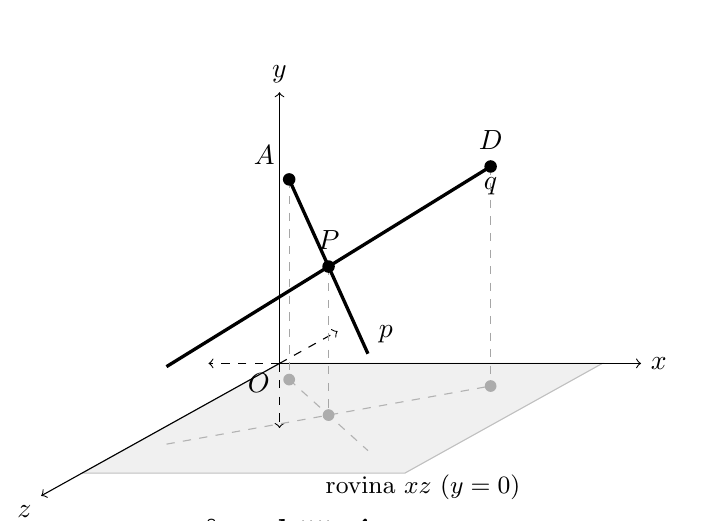
\begin{tikzpicture}[scale=0.82]
            \path[use as bounding box] (-3.9,-2.0) rectangle (6.1,5.2);
            \node[font=\bfseries\large, anchor=west] at (-1.6,-2.6) {různoběžné};

            \begin{scope}[space axes]
                \DrawSpaceBase

                % body
                \coordinate (P) at (2.2,2.3,1.6);
                \coordinate (A) at (0.6,3.1,0.5);
                \coordinate (B) at (3.8,1.5,2.7);

                \coordinate (C) at (0.5,1.2,2.5);
                \coordinate (D) at (3.9,3.4,0.7);

                % průměty
                \coordinate (Pp) at (2.2,0,1.6);
                \coordinate (Ap) at (0.6,0,0.5);
                \coordinate (Bp) at (3.8,0,2.7);
                \coordinate (Cp) at (0.5,0,2.5);
                \coordinate (Dp) at (3.9,0,0.7);

                % průměty přímek do roviny
                \draw[projline] (Ap) -- (Bp);
                \draw[projline] (Cp) -- (Dp);

                % přímky
                \draw[line3d] (A) -- (B) node[above right] {$p$};
                \draw[line3d] (C) -- (D) node[below] {$q$};

                % promítání bodů
                \draw[proj] (A) -- (Ap);
                \draw[proj] (P) -- (Pp);
                \draw[proj] (D) -- (Dp);

                % body v prostoru
                \node[point3d, label=above left:$A$] at (A) {};
                \node[point3d, label=above:$P$] at (P) {};
                \node[point3d, label=above:$D$] at (D) {};

                % body v rovině
                \node[pointproj] at (Ap) {};
                \node[pointproj] at (Pp) {};
                \node[pointproj] at (Dp) {};
            \end{scope}
        \end{tikzpicture}
    \end{minipage}
    \hfill
    %==================================================
    % ROVNOBĚŽNÉ
    %==================================================
    \begin{minipage}{0.48\textwidth}
        \centering
        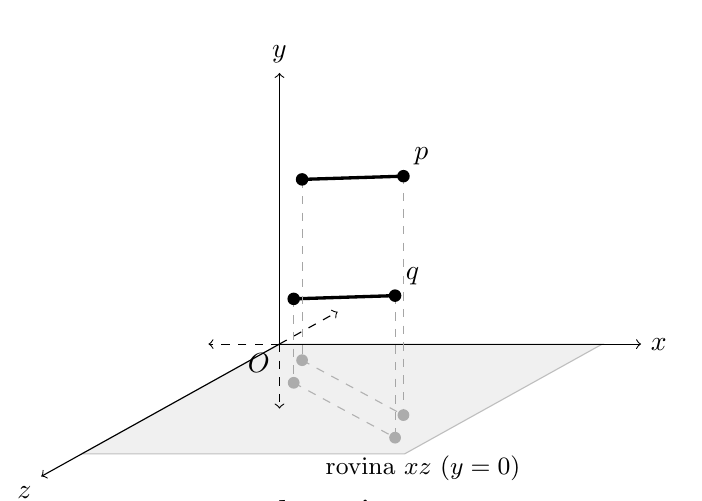
\begin{tikzpicture}[scale=0.82]
            \path[use as bounding box] (-3.9,-2.0) rectangle (6.1,4.9);
            \node[font=\bfseries\large, anchor=west] at (-1.6,-2.6) {rovnoběžné};

            \begin{scope}[space axes]
                \DrawSpaceBase

                % body
                \coordinate (A) at (0.8,2.8,0.5);
                \coordinate (B) at (3.9,3.7,2.2);

                \coordinate (C) at (1.3,1.3,1.2);
                \coordinate (D) at (4.4,2.2,2.9);

                % průměty
                \coordinate (Ap) at (0.8,0,0.5);
                \coordinate (Bp) at (3.9,0,2.2);
                \coordinate (Cp) at (1.3,0,1.2);
                \coordinate (Dp) at (4.4,0,2.9);

                % průměty přímek
                \draw[projline] (Ap) -- (Bp);
                \draw[projline] (Cp) -- (Dp);

                % přímky
                \draw[line3d] (A) -- (B) node[above right] {$p$};
                \draw[line3d] (C) -- (D) node[above right] {$q$};

                % promítání bodů
                \draw[proj] (A) -- (Ap);
                \draw[proj] (B) -- (Bp);
                \draw[proj] (C) -- (Cp);
                \draw[proj] (D) -- (Dp);

                % body v prostoru
                \node[point3d] at (A) {};
                \node[point3d] at (B) {};
                \node[point3d] at (C) {};
                \node[point3d] at (D) {};

                % body v rovině
                \node[pointproj] at (Ap) {};
                \node[pointproj] at (Bp) {};
                \node[pointproj] at (Cp) {};
                \node[pointproj] at (Dp) {};
            \end{scope}
        \end{tikzpicture}
    \end{minipage}

    \vspace{0.8em}

    %==================================================
    % TOTOŽNÉ
    %==================================================
    \begin{minipage}{0.48\textwidth}
        \centering
        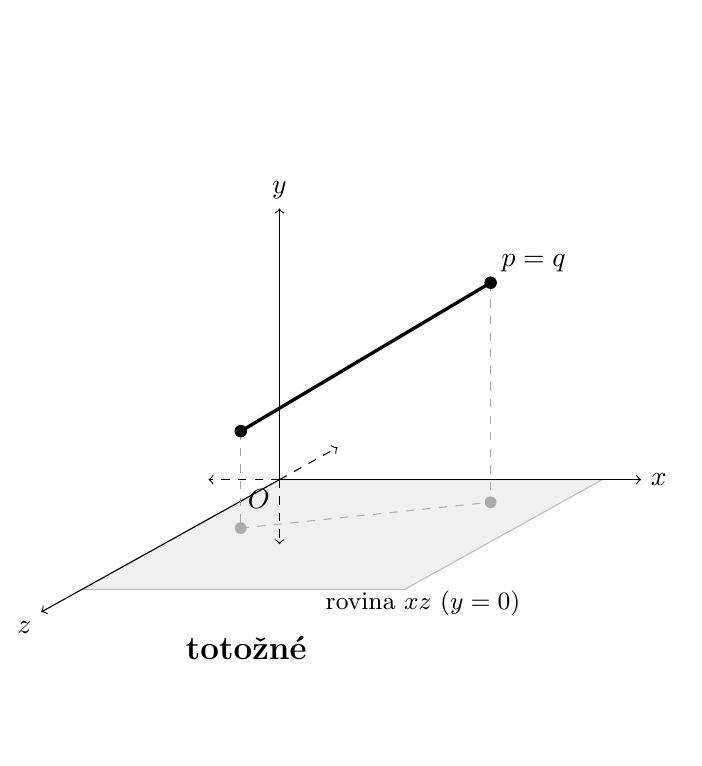
\begin{tikzpicture}[scale=0.82]
            \path[use as bounding box] (-3.9,-4.0) rectangle (6.1,7);
            \node[font=\bfseries\large, anchor=west] at (-1.6,-2.6) {totožné};

            \begin{scope}[space axes]
                \DrawSpaceBase

                % body na jedné přímce
                \coordinate (A) at (0.75,1.5,1.5);
                \coordinate (D) at (3.9,3.4,0.7);

                % průměty
                \coordinate (Ap) at (0.75,0,1.5);
                \coordinate (Dp) at (3.9,0,0.7);

                % průmět přímky
                \draw[projline] (Ap) -- (Dp);

                % přímka
                \draw[line3d] (A) -- (D) node[above right] {$p=q$};

                % promítání bodů
                \draw[proj] (A) -- (Ap);
                \draw[proj] (D) -- (Dp);

                % body v prostoru
                \node[point3d] at (A) {};
                \node[point3d] at (D) {};

                % body v rovině
                \node[pointproj] at (Ap) {};
                \node[pointproj] at (Dp) {};
            \end{scope}
        \end{tikzpicture}
    \end{minipage}
    \hfill
    %==================================================
    % MIMOBĚŽNÉ
    %==================================================
    \begin{minipage}{0.48\textwidth}
        \centering
        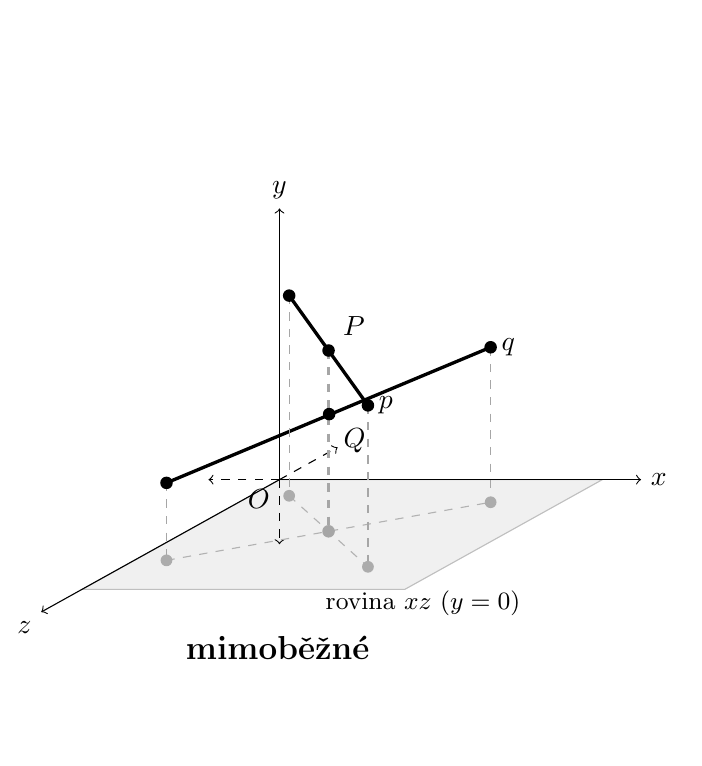
\begin{tikzpicture}[scale=0.82]
            \path[use as bounding box] (-3.9,-4.0) rectangle (6.1,7);
            \node[font=\bfseries\large, anchor=west] at (-1.6,-2.6) {mimoběžné};

            \begin{scope}[space axes]
                \DrawSpaceBase

                % body
                \coordinate (A) at (0.6,3.1,0.5);
                \coordinate (B) at (3.8,2.5,2.7);

                \coordinate (C) at (0.5,1.2,2.5);
                \coordinate (D) at (3.9,2.4,0.7);

                \coordinate (P1) at (2.2,2.8,1.6);
                \coordinate (P2) at (2.2,1.81,1.59);

                % průměty
                \coordinate (Aq) at (0.6,0,0.5);
                \coordinate (Bq) at (3.8,0,2.7);
                \coordinate (Cp) at (0.5,0,2.5);
                \coordinate (Dp) at (3.9,0,0.7);
                \coordinate (Pp) at (2.2,0,1.6);


                % průměty přímek
                \draw[projline] (Aq) -- (Bq);
                \draw[projline] (Cp) -- (Dp);

                % přímky
                \draw[line3d] (A) -- (B) node[right] {$p$};
                \draw[line3d] (C) -- (D) node[right] {$q$};
                \draw[line3d, dashed, gray!70] (P1) -- (Pp);

                % promítání bodů
                \draw[proj] (A) -- (Aq);
                \draw[proj] (B) -- (Bq);
                \draw[proj] (C) -- (Cp);
                \draw[proj] (D) -- (Dp);

                % body v prostoru
                \node[point3d] at (A) {};
                \node[point3d] at (B) {};
                \node[point3d] at (C) {};
                \node[point3d] at (D) {};
                \node[point3d, label=above right:{$P$}] at (P1) {};
                \node[point3d, label=below right:{$Q$}] at (P2) {};
                \node[point3d, gray!70] at (Pp) {};

                % body v rovině
                \node[pointproj] at (Aq) {};
                \node[pointproj] at (Bq) {};
                \node[pointproj] at (Cp) {};
                \node[pointproj] at (Dp) {};
            \end{scope}
        \end{tikzpicture}
    \end{minipage}

    \caption{Možné vzájemné polohy dvou přímek v prostoru.}
    \label{fig:Relative_positions_lines_space}
\end{figure}

Při určování vzájemné polohy budeme stejně jako v rovině nejprve
porovnávat směrové vektory přímek.

Jestliže existuje nenulové číslo $k\in\mathbb{R}$ takové, že
\[
    \vec{v}=k\vec{u},
\]
jsou směrové vektory rovnoběžné a obě přímky mají stejný směr.
V takovém případě mohou být přímky pouze \textbf{rovnoběžné}
nebo \textbf{totožné}. K rozlišení těchto možností stačí ověřit,
zda jeden bod jedné přímky leží také na druhé přímce.

Jestliže směrové vektory $\vec{u}$ a $\vec{v}$ rovnoběžné nejsou,
mají přímky různé směry. V rovině bychom již z této skutečnosti mohli
usoudit, že jsou přímky různoběžné. V prostoru to však neplatí.
Přímky mohou být buď \textbf{různoběžné}, nebo
\textbf{mimoběžné}.

Musíme proto zjistit, zda mají společný bod.

Společný bod musí současně vyhovovat parametrickému vyjádření obou
přímek. Musí tedy existovat hodnoty parametrů $t$ a $s$, pro které
platí
\[
    A+t\vec{u}=B+s\vec{v}.
\]

Jsou-li
\[
    A[x_A;y_A;z_A],
    \qquad
    B[x_B;y_B;z_B],
\]
\[
    \vec{u}=(u_x;u_y;u_z),
    \qquad
    \vec{v}=(v_x;v_y;v_z),
\]
dostáváme soustavu tří rovnic o dvou neznámých parametrech $t$ a $s$:
\begin{equation}
    \begin{cases}
        x_A+t u_x=x_B+s v_x,\\
        y_A+t u_y=y_B+s v_y,\\
        z_A+t u_z=z_B+s v_z.
    \end{cases}
    \label{eq:Intersection_parametric_lines_space}
\end{equation}

Má-li tato soustava řešení, existuje společný bod obou přímek
a přímky jsou různoběžné. Nemá-li soustava řešení, přímky se
neprotínají, a protože jejich směrové vektory nejsou rovnoběžné,
jsou přímky mimoběžné.

Celý rozhodovací postup můžeme shrnout následovně:
\[
\begin{array}{c|c}
\text{Podmínka}
&
\text{Vzájemná poloha přímek}
\\
\hline
\vec{v}=k\vec{u},\ k\neq0,\ B\in p
&
\text{přímky jsou totožné}
\\[1mm]
\vec{v}=k\vec{u},\ k\neq0,\ B\notin p
&
\text{přímky jsou rovnoběžné}
\\[1mm]
\vec{u}\not\parallel\vec{v}
\text{ a soustava \eqref{eq:Intersection_parametric_lines_space} má řešení}
&
\text{přímky jsou různoběžné}
\\[1mm]
\vec{u}\not\parallel\vec{v}
\text{ a soustava \eqref{eq:Intersection_parametric_lines_space} nemá řešení}
&
\text{přímky jsou mimoběžné}
\end{array}
\]

Rozhodovací postup můžeme znázornit také pomocí schématu na obrázku
\ref{fig:Relative_position_parametric_lines_space_decision}.

\begin{figure}[H]
    \centering
    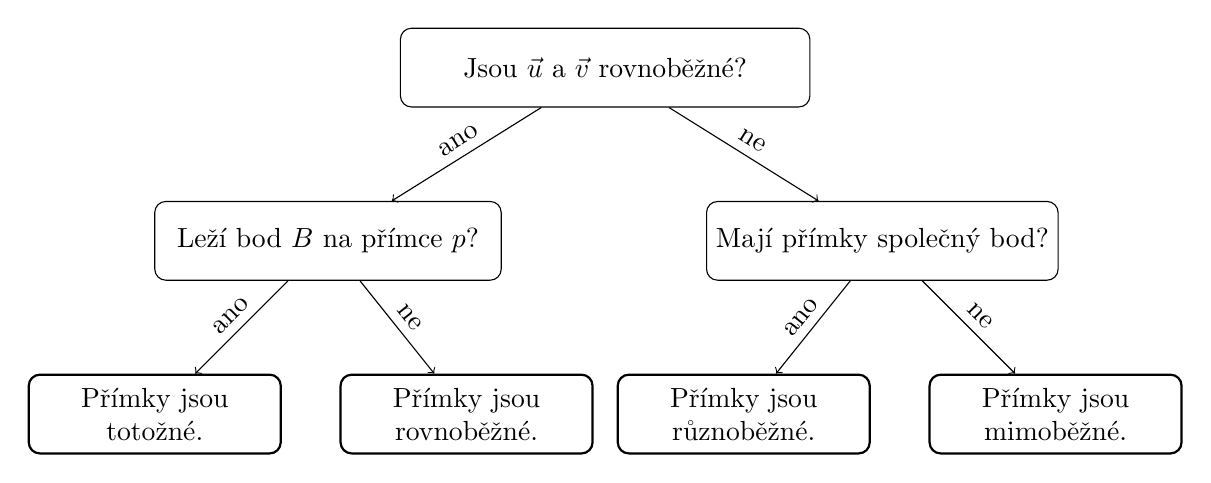
\begin{tikzpicture}[scale=0.88, every node/.style={align=center}]

        % Uzly
        \node[
            draw,
            rounded corners,
            minimum width=5.2cm,
            minimum height=1cm
        ]
        (start) at (0,0)
        {Jsou $\vec{u}$ a $\vec{v}$ rovnoběžné?};

        \node[
            draw,
            rounded corners,
            minimum width=4.4cm,
            minimum height=1cm
        ]
        (point) at (-4,-2.5)
        {Leží bod $B$ na přímce $p$?};

        \node[
            draw,
            rounded corners,
            minimum width=4.4cm,
            minimum height=1cm
        ]
        (intersection) at (4,-2.5)
        {Mají přímky společný bod?};

        \node[
            draw,
            rounded corners,
            minimum width=3.2cm,
            minimum height=1cm,
            thick
        ]
        (coincident) at (-6.5,-5)
        {Přímky jsou\\totožné.};

        \node[
            draw,
            rounded corners,
            minimum width=3.2cm,
            minimum height=1cm,
            thick
        ]
        (parallel) at (-2,-5)
        {Přímky jsou\\rovnoběžné.};

        \node[
            draw,
            rounded corners,
            minimum width=3.2cm,
            minimum height=1cm,
            thick
        ]
        (intersecting) at (2,-5)
        {Přímky jsou\\různoběžné.};

        \node[
            draw,
            rounded corners,
            minimum width=3.2cm,
            minimum height=1cm,
            thick
        ]
        (skew) at (6.5,-5)
        {Přímky jsou\\mimoběžné.};

        % Šipky
        \draw[->] (start) -- (point)
            node[midway, above, sloped] {ano};

        \draw[->] (start) -- (intersection)
            node[midway, above, sloped] {ne};

        \draw[->] (point) -- (coincident)
            node[midway, above, sloped] {ano};

        \draw[->] (point) -- (parallel)
            node[midway, above, sloped] {ne};

        \draw[->] (intersection) -- (intersecting)
            node[midway, above, sloped] {ano};

        \draw[->] (intersection) -- (skew)
            node[midway, above, sloped] {ne};

    \end{tikzpicture}
    \caption{Postup při určování vzájemné polohy parametricky zadaných
    přímek v prostoru.}
    \label{fig:Relative_position_parametric_lines_space_decision}
\end{figure}

\begin{remark}
    Při hledání průsečíku je důležité ověřit \textbf{všechny tři rovnice}
    soustavy~\eqref{eq:Intersection_parametric_lines_space}.
    Vyřešením dvou rovnic můžeme získat konkrétní hodnoty parametrů
    $t$ a $s$, ale tyto hodnoty ještě musí vyhovovat také třetí rovnici.

    Právě v této třetí rovnici se často projeví rozdíl mezi různoběžnými
    a mimoběžnými přímkami.
\end{remark}


\subsubsection{Rovnoběžné přímky}
\label{subsubsec:Parallel_parametric_lines_space}

Jsou-li směrové vektory dvou přímek navzájem rovnoběžné, nemůžeme
pouze z této skutečnosti rozhodnout, zda jsou přímky rovnoběžné,
nebo totožné. Musíme ještě zjistit, zda mají některý bod společný.

\begin{example}
    \label{exa:Parallel_parametric_lines_space}
    Určete vzájemnou polohu přímek $p$ a $q$ zadaných bodem
    a směrovým vektorem:
    \[
        p:\ A[-1;3;2],
        \qquad
        \vec{u}=(-1;2;1),
    \]
    \[
        q:\ B[1;1;0],
        \qquad
        \vec{v}=(2;-4;-2).
    \]

    Nejprve porovnáme směrové vektory. Platí
    \[
        \vec{v}
        =
        (2;-4;-2)
        =
        -2(-1;2;1)
        =
        -2\vec{u}.
    \]

    Směrové vektory jsou tedy rovnoběžné. Přímky $p$ a $q$ jsou
    proto buď rovnoběžné, nebo totožné.

    Ověříme, zda například bod $A[-1;3;2]$ leží na přímce $q$.
    Parametrické vyjádření přímky $q$ je
    \[
        \begin{aligned}
            q: x&=1+2s,\\
            y&=1-4s,\\
            z&=-2s; s\in\mathbb{R}.
        \end{aligned}
    \]

    Dosadíme souřadnice bodu $A$:
    \begin{align*}
        -1&=1+2s
        &&\Rightarrow s=-1,\\
        3&=1-4s
        &&\Rightarrow s=-\frac12,\\
        2&=-2s
        &&\Rightarrow s=-1.
    \end{align*}

    Z jednotlivých rovnic nevychází stejná hodnota parametru.
    Bod $A$ proto na přímce $q$ neleží.

    Přímky mají rovnoběžné směrové vektory, ale nemají žádný
    společný bod. Jsou tedy rovnoběžné:
    \[
        p\parallel q.
    \]
\end{example}

\begin{example}
    \label{exa:Parallel_line_through_origin_space}
    Je dána přímka $p=\left\{\left[2;-1;4\right] + t\left(-3;2;1\right) ; t\in\mathbb{R}\right\}$.
    Určete parametrické vyjádření přímky $q$, která je rovnoběžná
    s přímkou $p$ a prochází počátkem soustavy souřadnic.

    Z parametrického vyjádření přímky $p$ určíme její směrový vektor
    \[
        \vec{u}=(-3;2;1).
    \]

    Má-li být přímka $q$ rovnoběžná s přímkou $p$, můžeme pro ni použít
    stejný směrový vektor, případně libovolný jeho nenulový násobek.

    Přímka $q$ má procházet počátkem soustavy souřadnic
    \[
        O[0;0;0].
    \]

    Použijeme tedy bod $O$ a směrový vektor
    \[
        \vec{u}=(-3;2;1).
    \]

    Parametrické vyjádření hledané přímky je
    \[
        \begin{aligned}
            q: x&=-3s,\\
            y&=2s,\\
            z&=s; s\in\mathbb{R}.
        \end{aligned}
    \]

    Přímky $p$ a $q$ mají stejné směrové vektory, a proto jsou
    rovnoběžné nebo totožné. Protože bod $O[0;0;0]$ na přímce $p$
    neleží, jsou přímky skutečně rovnoběžné:
    \[
        p\parallel q.
    \]
\end{example}

\subsubsection{Různoběžné přímky a jejich průsečík}
\label{subsubsec:Intersecting_parametric_lines_space}

Nejsou-li směrové vektory dvou přímek rovnoběžné, mají přímky
různé směry. Abychom rozhodli, zda jsou různoběžné, nebo mimoběžné,
musíme zjistit, zda mají společný bod.

Průsečík musí současně ležet na obou přímkách. Jeho souřadnice proto
musí vzniknout pro určitou hodnotu parametru $t$ na přímce $p$
a současně pro určitou hodnotu parametru $s$ na přímce $q$.

\begin{remark}
    Stejně jako v rovině musíme při porovnávání dvou parametricky
    vyjádřených přímek používat dva různé parametry:
    \[
        p:\ X=A+t\vec{u},
        \qquad
        q:\ X=B+s\vec{v}.
    \]

    Hodnoty $t$ a $s$ obecně nejsou stejné. Vyjadřují totiž dvě
    různá posunutí ze dvou různých zvolených bodů a pomocí dvou
    různých směrových vektorů.
\end{remark}

\begin{example}
    \label{exa:Intersecting_parametric_lines_space}
    Určete vzájemnou polohu přímek
    \[
        \begin{aligned}
            p: x&=-3+2t,\\
            y&=-1+t,\\
            z&=1; t\in\mathbb{R}
        \end{aligned}
    \]
    a
    \[
        \begin{aligned}
            q: x&=2+s,\\
            y&=-2-3s,\\
            z&=-1-2s; s\in\mathbb{R}.
        \end{aligned}
    \]
    Jsou-li přímky různoběžné, určete jejich průsečík.

    Směrové vektory přímek jsou
    \[
        \vec{u}=(2;1;0),
        \qquad
        \vec{v}=(1;-3;-2).
    \]

    Tyto vektory nejsou rovnoběžné, protože neexistuje číslo
    $k\in\mathbb{R}$, pro které by platilo
    \[
        (1;-3;-2)=k(2;1;0).
    \]

    Přímky jsou tedy buď různoběžné, nebo mimoběžné.
    Pokusíme se najít jejich společný bod.

    Položíme odpovídající souřadnice sobě rovny:
    \begin{align*}
        -3+2t &= 2+s,\\
        -1+t &= -2-3s,\\
        1 &= -1-2s.
    \end{align*}

    Ze třetí rovnice získáme
    \[
        2=-2s
        \qquad\Rightarrow\qquad
        s=-1.
    \]

    Dosadíme tuto hodnotu do první rovnice:
    \begin{align*}
        -3+2t &= 2-1,\\
        -3+2t &= 1,\\
        2t &= 4,\\
        t &= 2.
    \end{align*}

    Nyní musíme ověřit také druhou rovnici:
    \[
        -1+2
        =
        -2-3(-1),
    \]
    tedy
    \[
        1=1.
    \]

    Všechny tři rovnice jsou splněny pro
    \[
        t=2,
        \qquad
        s=-1.
    \]

    Přímky tedy mají společný bod a jsou různoběžné.

    Jeho souřadnice získáme například dosazením $t=2$
    do parametrického vyjádření přímky $p$:
    \begin{align*}
        x&=-3+2\cdot2=1,\\
        y&=-1+2=1,\\
        z&=1.
    \end{align*}

    Průsečíkem přímek je bod
    \[
        P[1;1;1].
    \]

    Zapisujeme
    \[
        p\cap q=\{P[1;1;1]\}.
    \]
\end{example}

\begin{remark}
    Hodnoty parametrů $t$ a $s$ nejsou souřadnicemi průsečíku.
    Určují pouze polohu společného bodu v parametrickém vyjádření
    jednotlivých přímek. Souřadnice průsečíku získáme až jejich
    dosazením do rovnic jedné z přímek.
\end{remark}

\begin{example}
    \label{exa:Perpendicular_lines_through_point_space}
    Je dána přímka
    \[
        \begin{aligned}
            p: x&=-3+2t,\\
            y&=-1+t,\\
            z&=1; t\in\mathbb{R}.
        \end{aligned}
    \]
    a bod $P[1;1;1]$, který na této přímce leží.

    Určete dvě různé přímky $q$ a $r$, které procházejí bodem $P$
    a jsou kolmé k přímce $p$.

    Napřed určíme směrový vektor přímky $p$, který je
    \[
        \vec{u}=(2;1;0).
    \]

    Aby byla přímka $q$ kolmá k přímce $p$, musí její směrový vektor
    $\vec{v}=(v_x;v_y;v_z)$ být kolmý ke směrovému vektoru
    $\vec{u}$. Musí tedy platit
    \[
        \vec{u}\cdot\vec{v}=0.
    \]

    Po dosazení získáme
    \[
        (2;1;0)\cdot(v_x;v_y;v_z)=0,
    \]
    tedy
    \[
        2v_x+v_y=0.
    \]

    Tato rovnice neurčuje směrový vektor jednoznačně. Protože dostáváme jednu rovnici o dvou neznámých,
    máme nekonečně mnoho řešení. Můžeme tedy jednu souřadnici libovolně zvolit, například
    zvolit $v_x=1$ a využít toho, že $v_z=0$ a dosadit potom do rovnice
    \[
        2\cdot1+v_y=0,
    \]
    a tedy
    \[
        v_y=-2.
    \]

    Jedním vhodným směrovým vektorem je proto
    \[
        \vec{v}=(1;-2;0).
    \]

    Přímka $q$ procházející bodem $P[1;1;1]$ má parametrické
    vyjádření
    \[
        \begin{aligned}
            q: x&=1+s,\\
            y&=1-2s,\\
            z&=1; s\in\mathbb{R}.
        \end{aligned}
    \]

    Můžeme však zvolit také například
    \[
        v_x=0,\qquad v_y=0,\qquad v_z=1,
    \]
    protože
    \[
        (2;1;0)\cdot(0;0;1)=0.
    \]

    Dostáváme tedy druhý směrový vektor
    \[
        \vec{w}=(0;0;1)
    \]
    a druhou kolmou přímku
    \[
        \begin{aligned}
            r: x&=1,\\
            y&=1,\\
            z&=1+\lambda; \lambda\in\mathbb{R}.
        \end{aligned}
    \]

    Obě přímky $q$ a $r$ procházejí bodem $P$, ve kterém protínají
    přímku $p$, a jejich směrové vektory jsou kolmé ke směrovému
    vektoru přímky $p$. Platí tedy
    \[
        q\perp p
        \qquad\text{a}\qquad
        r\perp p.
    \]
\end{example}

\begin{remark}
    V rovině prochází daným bodem přímky právě jedna přímka, která je
    k této přímce kolmá. V prostoru je situace jiná.

    Pro směrový vektor
    \[
        \vec{u}=(2;1;0)
    \]
    musí směrový vektor každé kolmé přímky splňovat pouze podmínku
    \[
        2v_x+v_y=0.
    \]
    Souřadnici $v_z$ můžeme volit libovolně a stejně tak můžeme volit
    jednu ze souřadnic $v_x$ a $v_y$ a druhou dopočítat. Existuje proto
    nekonečně mnoho různých směrů kolmých k vektoru $\vec{u}$.

    Bodem $P$ tak v prostoru prochází nekonečně mnoho přímek kolmých
    k přímce $p$. Všechny tyto přímky společně vyplňují jednu rovinu,
    která prochází bodem $P$ a je kolmá k přímce $p$.

    S touto rovinou a jejím analytickým popisem se seznámíme později.
\end{remark}

\subsubsection{Mimoběžné přímky}
\label{subsubsec:Skew_parametric_lines_space}

Mimoběžné přímky mají různé směry, ale nemají žádný společný bod.
Při jejich určování proto nejprve zjistíme, že jejich směrové vektory
nejsou rovnoběžné, a poté ověříme, že soustava rovnic pro společný bod
nemá řešení.

\begin{example}
    \label{exa:Skew_parametric_lines_space}
    Určete vzájemnou polohu přímek $p=\left\{\left[2;3;-1\right] + t\left(1;-2;1\right); t\in\mathbb{R}\right\}$
    a
    \[
        \begin{aligned}
            q: x&=-2+3s,\\
            y&=3+2s,\\
            z&=3+s; s\in\mathbb{R}.
        \end{aligned}
    \]

    Směrové vektory přímek jsou
    \[
        \vec{u_p}=(1;-2;1),
        \qquad
        \vec{v_q}=(3;2;1).
    \]

    Směrové vektory nejsou rovnoběžné, protože neexistuje číslo
    $k\in\mathbb{R}$ takové, že
    \[
        \vec{v_q}=k\vec{u_p}.
    \]

    Přímky mohou být různoběžné nebo mimoběžné. Zjistíme tedy,
    zda mají společný bod.

    Položíme odpovídající souřadnice sobě rovny:
    \begin{align*}
        2+t &= -2+3s,\\
        3-2t &= 3+2s,\\
        -1+t &= 3+s.
    \end{align*}

    Ze třetí rovnice vyjádříme parametr $t$:
    \[
        t=s+4.
    \]

    Dosadíme jej do první rovnice:
    \begin{align*}
        2+(s+4) &= -2+3s,\\
        6+s &= -2+3s,\\
        8 &= 2s,\\
        s &= 4.
    \end{align*}

    Nyní však musíme zkontrolovat také druhou rovnici.
    Dosadíme do ní $t=s+4$:
    \begin{align*}
        3-2(s+4) &= 3+2s,\\
        3-2s-8 &= 3+2s,\\
        -5-2s &= 3+2s,\\
        -8 &= 4s,\\
        s &= -2.
    \end{align*}

    Z první a druhé rovnice jsme po použití třetí rovnice získali
    dvě různé hodnoty parametru:
    \[
        s=4
        \qquad\text{a}\qquad
        s=-2.
    \]

    Neexistuje tedy dvojice parametrů $t$ a $s$, která by současně
    splňovala všechny tři rovnice. Přímky nemají společný bod.

    Protože zároveň nemají rovnoběžné směrové vektory, jsou
    \textbf{mimoběžné}.
\end{example}

\begin{remark}
    Právě u mimoběžných přímek je obzvlášť důležité nepřestat
    s výpočtem po vyřešení pouze dvou rovnic. Dvě rovnice o dvou
    neznámých mohou mít řešení, ale třetí rovnice může ukázat,
    že nalezená dvojice parametrů společnému bodu obou přímek
    neodpovídá.
\end{remark}

\begin{example}
    \label{exa:Construct_skew_line_space}

    Je dána přímka $p=\left\{\left[2;3;-1\right] + t\left(1;-2;1\right); t\in\mathbb{R}\right\}$.
    Určete parametrické vyjádření přímky $q$, která prochází bodem $B[0;1;2]$ a je rovnoběžná s osou $z$. 
    Poté určete vzájemnou polohu přímek $p$ a $q$.

    Přímka rovnoběžná s osou $z$ má směrový vektor například
    \[
        \vec{v}=(0;0;1).
    \]

    Protože má přímka $q$ procházet bodem $B[0;1;2]$, dostáváme tedy přímku $q=B+s\cdot \vec{v}$ můžeme ji
    zapsat parametricky ve tvaru
    \[
        \begin{aligned}
            q: x&=0,\\
            y&=1,\\
            z&=2+s; s\in\mathbb{R}.
        \end{aligned}
    \]

    Směrový vektor přímky $p$ je
    \[
        \vec{u}=(1;-2;1).
    \]

    Vektory
    \[
        \vec{u}=(1;-2;1)
        \qquad\text{a}\qquad
        \vec{v}=(0;0;1)
    \]
    nejsou rovnoběžné. Přímky $p$ a $q$ tedy mohou být různoběžné
    nebo mimoběžné.

    Zjistíme, zda mají společný bod. Položíme odpovídající souřadnice
    sobě rovny:
    \[
        \begin{cases}
            2+t=0,\\
            3-2t=1,\\
            -1+t=2+s.
        \end{cases}
    \]

    Z první rovnice dostáváme
    \[
        t=-2.
    \]

    Po dosazení do druhé rovnice však získáme
    \[
        3-2(-2)=1,
    \]
    tedy
    \[
        7=1,
    \]
    což není pravda.

    Přímky proto nemají společný bod. Protože současně nejsou
    rovnoběžné, jsou \textbf{mimoběžné}.
\end{example}

\begin{example}
    \label{exa:Line_intersecting_q_parallel_p}

    Jsou dány mimoběžné přímky
    \[
        \begin{aligned}
            p: x&=2+t,\\
            y&=3-2t,\\
            z&=-1+t; t\in\mathbb{R}
        \end{aligned}
    \]
    a
    \[
        \begin{aligned}
            q: x&=-2+3s,\\
            y&=3+2s,\\
            z&=3+s; s\in\mathbb{R}.
        \end{aligned}
    \]

    Najděte přímku $r$, která je rovnoběžná s přímkou $p$
    a zároveň je různoběžná s přímkou $q$.

    Směrový vektor přímky $p$ je
    \[
        \vec{u}=(1;-2;1).
    \]

    Má-li být přímka $r$ rovnoběžná s přímkou $p$, můžeme jako její
    směrový vektor použít právě vektor
    \[
        \vec{u}=(1;-2;1).
    \]

    Zároveň chceme, aby přímka $r$ protínala přímku $q$.
    Zvolíme proto libovolný bod na přímce $q$.
    Nejjednodušší je položit
    \[
        s=0.
    \]

    Dostáváme bod
    \[
        B[-2;3;3].
    \]

    Přímka $r$ procházející bodem $B$ a mající směrový vektor
    $\vec{u}=(1;-2;1)$ má tedy parametrické vyjádření
    \[
        \begin{aligned}
            r: x&=-2+\lambda,\\
            y&=3-2\lambda,\\
            z&=3+\lambda; \lambda\in\mathbb{R}.
        \end{aligned}
    \]

    Přímky $p$ a $r$ mají stejné směrové vektory, proto
    \[
        r\parallel p.
    \]

    Přímka $r$ zároveň prochází bodem $B[-2;3;3]$, který leží také
    na přímce $q$. Platí tedy
    \[
        r\cap q=\{B\}.
    \]

    Směrový vektor přímky $q$ je
    \[
        \vec{v}=(3;2;1),
    \]
    který není rovnoběžný s vektorem
    \[
        \vec{u}=(1;-2;1).
    \]

    Přímky $q$ a $r$ tedy mají právě jeden společný bod, a jsou proto
    \textbf{různoběžné}.

    Hledaná přímka může být například
    \[
        \begin{aligned}
            r: x&=-2+\lambda,\\
            y&=3-2\lambda,\\
            z&=3+\lambda; \lambda\in\mathbb{R}.
        \end{aligned}
    \]
\end{example}

\begin{remark}
    Hledaná přímka $r$ není určena jednoznačně.

    V předchozím příkladu jsme zvolili bod přímky $q$ odpovídající
    hodnotě $s=0$. Mohli bychom však zvolit libovolnou jinou hodnotu
    parametru $s$.

    Obecný bod přímky $q$ má souřadnice
    \[
        Q_s[-2+3s;3+2s;3+s].
    \]

    Každým takovým bodem můžeme vést přímku se směrovým vektorem
    přímky $p$,
    \[
        \vec{u}=(1;-2;1).
    \]

    Dostáváme tak celou soustavu přímek
    \[
        \begin{aligned}
            r_s: x&=-2+3s+\lambda,\\
            y&=3+2s-2\lambda,\\
            z&=3+s+\lambda;
            \qquad s,\lambda\in\mathbb{R}.
        \end{aligned}
    \]

    Pro každou pevně zvolenou hodnotu $s$ dostaneme jednu přímku
    $r_s$, která protíná přímku $q$ a je rovnoběžná s přímkou $p$.

    Takových přímek tedy existuje nekonečně mnoho.

    Zajímavé je, že všechny tyto přímky společně vyplňují jednu
    rovinu. Ta obsahuje přímku $q$ a je rovnoběžná s přímkou $p$.
    S takovým popisem roviny se seznámíme opět v následujících kapitolách.
\end{remark}


\subsubsection{Totožné přímky}
\label{subsubsec:Coincident_parametric_lines_space}

Jsou-li směrové vektory dvou přímek rovnoběžné a zároveň jeden bod
první přímky leží na druhé přímce, mají přímky stejný směr i společný
bod. V takovém případě představují tutéž množinu bodů a jsou totožné.

\begin{example}
    \label{exa:Coincident_parametric_lines_space}
    Určete vzájemnou polohu přímek
    \[
        \begin{aligned}
            p: x&=-3+4t,\\
            y&=4-2t,\\
            z&=2+2t; t\in\mathbb{R}
        \end{aligned}
    \]
    a
    \[
        \begin{aligned}
            q: x&=1-6s,\\
            y&=2+3s,\\
            z&=4-3s; s\in\mathbb{R}.
        \end{aligned}
    \]

    Z parametrických rovnic vyčteme směrové vektory
    \[
        \vec{u}=(4;-2;2),
        \qquad
        \vec{v}=(-6;3;-3).
    \]

    Platí
    \[
        \vec{v}
        =
        -\frac32\vec{u},
    \]
    takže směrové vektory jsou rovnoběžné.

    Přímky jsou tedy buď rovnoběžné, nebo totožné.

    Přímka $q$ prochází například bodem
    \[
        B[1;2;4],
    \]
    který získáme pro $s=0$.

    Ověříme, zda tento bod leží také na přímce $p$:
    \begin{align*}
        1&=-3+4t
        &&\Rightarrow t=1,\\
        2&=4-2t
        &&\Rightarrow t=1,\\
        4&=2+2t
        &&\Rightarrow t=1.
    \end{align*}

    Ze všech tří rovnic vyšla stejná hodnota parametru $t=1$.
    Bod $B$ tedy leží na přímce $p$.

    Přímky mají rovnoběžné směrové vektory a společný bod,
    a proto jsou totožné:
    \[
        p=q.
    \]

    Jejich průnikem je celá přímka:
    \[
        p\cap q=p=q.
    \]
\end{example}

Vzájemnou polohu dvou parametricky vyjádřených přímek v prostoru
tedy určujeme ve dvou krocích. Nejprve porovnáme jejich směrové
vektory. Jsou-li rovnoběžné, rozhodujeme mezi rovnoběžnými a
totožnými přímkami pomocí společného bodu. Nejsou-li rovnoběžné,
hledáme průsečík. Podle toho, zda společný bod existuje, jsou
přímky různoběžné, nebo mimoběžné.

\begin{example}
    \label{exa:Parametric_z_axis}
    Určete parametrické vyjádření osy $z$.

    Osa $z$ prochází počátkem soustavy souřadnic
    \[
        O[0;0;0]
    \]
    a její směr je určen například vektorem
    \[
        \vec{u}=(0;0;1).
    \]

    Použijeme vztah
    \[
        X=O+t\vec{u}.
    \]
    Dostáváme
    \[
        [x;y;z]
        =
        [0;0;0]+t(0;0;1),
    \]
    a tedy
    \[
        \begin{aligned}
            z: x&=0,\\
            y&=0,\\
            z&=t; t\in\mathbb{R}.
        \end{aligned}
    \]

    Osa $z$ je tedy tvořena právě body, jejichž první dvě souřadnice
    jsou nulové a třetí souřadnice může nabývat libovolné reálné hodnoty.
\end{example}

\begin{example}
    \label{exa:Relative_position_lines_cube}
    Je dána krychle $ABCDEFGH$ o hraně délky $4$, přičemž $A[0;0;4], B[4;0;4],$ 
    
    $H[0;4;0]$.
    Body $K,L,M,N,P,Q$ jsou po řadě středy hran
    $AB$, $BF$, $BC$, $GH$, $AE$, $EH$.
    a bod $R$ leží na hraně $AB$ tak, že $|AR|=1$.

    \begin{figure}[H]
        \centering
        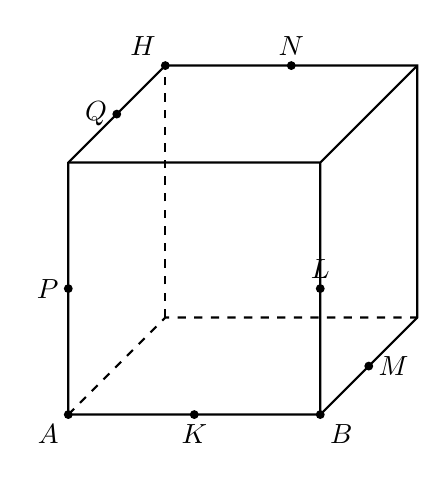
\begin{tikzpicture}[scale=0.8]
            % Vrcholy krychle
            \coordinate (A) at (0,0,4);
            \coordinate (B) at (4,0,4);
            \coordinate (C) at (4,0,0);
            \coordinate (D) at (0,0,0);
            \coordinate (E) at (0,4,4);
            \coordinate (F) at (4,4,4);
            \coordinate (G) at (4,4,0);
            \coordinate (H) at (0,4,0);

            % Středové body hran
            \coordinate (K) at (2,0,4);
            \coordinate (L) at (4,2,4);
            \coordinate (M) at (4,0,2);
            \coordinate (N) at (2,4,0);
            \coordinate (P) at (0,2,4);
            \coordinate (Q) at (0,4,2);

            % Hrany krychle
            \draw[thick] (A) -- (B) -- (C) -- (G) -- (H) -- (E) -- (A);
            \draw[thick] (E) -- (F) -- (B) -- (F) -- (G);
            \draw[dashed, thick] (A) -- (D) -- (C);
            \draw[dashed, thick] (D) -- (H);

            % Body A, B, H
            \fill (A) circle (2pt) node[below left] {$A$};
            \fill (B) circle (2pt) node[below right] {$B$};
            \fill (H) circle (2pt) node[above left] {$H$};

            % Body K, L, M, N, P, Q, R
            \fill (K) circle (2pt) node[below] {$K$};
            \fill (L) circle (2pt) node[above] {$L$};
            \fill (M) circle (2pt) node[right] {$M$};
            \fill (N) circle (2pt) node[above] {$N$};
            \fill (P) circle (2pt) node[left] {$P$};
            \fill (Q) circle (2pt) node[left] {$Q$};

        \end{tikzpicture}
        \caption{Krychle a vyznačené body k příkladu.}
    \end{figure}

    Určete vzájemnou polohu přímek
    \begin{enumerate}[label=\alph*)]
        \item $KL$ a $MN$,
        \item $AK$ a $EM$,
        \item $KQ$ a $CN$,
        \item $KP$ a $CH$,
        \item $AQ$ a $CN$.
    \end{enumerate}

    Nejprve určíme souřadnice bodů, které budeme v jednotlivých částech
    potřebovat. Z daných souřadnic vrcholů krychle dostáváme
    \[
        D[0;0;0],\qquad E[0;4;4],\qquad
        C[4;0;4],\qquad F[4;4;4],\qquad G[4;4;0].
    \]
    Protože body $K,L,M,N,P,Q$ jsou středy příslušných hran, platí
    \[
        K[2;0;4],\qquad L[4;2;4],\qquad M[4;0;2],
    \]
    \[
        N[2;4;0],\qquad P[0;2;4],\qquad Q[0;4;2].
    \]

    \textbf{a) Určeme vzájemnou polohu přímek $KL$ a $MN$.}

    Směrový vektor přímky $KL$ je
    \[
        \overrightarrow{KL}
        =L-K
        =(4-2;2-0;4-4)
        =(2;2;0).
    \]

    Směrový vektor přímky $MN$ je
    \[
        \overrightarrow{MN}
        =N-M
        =(2-4;4-0;0-4)
        =(-2;4;-4).
    \]

    Směrové vektory nejsou násobky, tudíž přímky nejsou rovnoběžné.
    Mohou být různoběžné, nebo mimoběžné. Zjistíme tedy, zda mají společný bod.

    \begin{align*}
        p_{KL}: x&=2+2t,\\
                y&=0+2t,\\
                z&=4+0t; t\in\mathbb{R},\\
        p_{MN}: x&=4-2s,\\
                y&=0+4s,\\
                z&=2-4s; s\in\mathbb{R}.
    \end{align*}

    Pro společný bod musí platit, že existují hodnoty parametrů $t$ a $s$, pro které současně platí
    \begin{align*}
        2+2t&=4-2s,\\
        0+2t&=0+4s,\\
        4+0t&=2-4s.
    \end{align*}

    Z druhé rovnice dostáváme:
    \[
    t=2s,
    \]
    Po dosazení do první rovnice dostáváme:
    \begin{align*}
        2+2(2s)&=4-2s,\\
        2+4s&=4-2s,\\
        6s&=2,\\
        s&=\frac13,
    \end{align*}

    Poté hodnota parametru $t$ je $t=\frac{2}{3}$. Ověříme třetí rovnici:
    \begin{align*}
        4+0\cdot\frac{2}{3}&=2-4\cdot\frac{1}{3},\\
        4&=2-\frac{4}{3},\\
        4&\neq\frac{2}{3},
    \end{align*}

    Soustava nemá řešení, přímky tedy nemají společný bod a protože jsou jejich směrové vektory různoběžné.
    Přímky $KL$ a $MN$ jsou tedy \textbf{mimoběžné}.

    \textbf{b) Určeme vzájemnou polohu přímek $AK$ a $EM$.}

    Směrový vektor přímky $AK$ je
    \[
        \overrightarrow{AK}
        =K-A
        =(2;0;0).
    \]

    Směrový vektor přímky $EM$ je
    \[
        \overrightarrow{EM}
        =M-E
        =(4;-4;-2).
    \]

    Směrové vektory nejsou rovnoběžné, 
    
    \[
        \begin{aligned}
            AK: x&=2t,\\
            y&=0,\\
            z&=0; t\in\mathbb{R},
        \end{aligned}
        \qquad
        \begin{aligned}
            EM: x&=2s,\\
            y&=4-4s,\\
            z&=4s; s\in\mathbb{R}.
        \end{aligned}
    \]

    Pro společný bod by muselo současně platit
    \[
        \begin{cases}
            2t=2s,\\
            0=4-4s,\\
            0=4s.
        \end{cases}
    \]

    Z druhé rovnice dostáváme
    \[
        s=1,
    \]
    zatímco ze třetí rovnice
    \[
        s=0.
    \]

    Soustava tedy nemá řešení. Přímky nemají společný bod a jejich
    směrové vektory nejsou rovnoběžné.

    Přímky $AK$ a $EM$ jsou proto \textbf{mimoběžné}.


    \textbf{c) Určeme vzájemnou polohu přímek $KQ$ a $CN$.}

    Směrový vektor přímky $KQ$ je
    \[
        \overrightarrow{KQ}
        =Q-K
        =(-2;4;2).
    \]

    Směrový vektor přímky $CN$ je
    \[
        \overrightarrow{CN}
        =N-C
        =(-2;4;-4).
    \]

    Směrové vektory nejsou rovnoběžné. Přímky jsou tedy buď
    různoběžné, nebo mimoběžné.

    Jejich parametrická vyjádření jsou například
    \[
        \begin{aligned}
            p_{KQ}: x&=2-2t,\\
                    y&=4t,\\
                    z&=2t; t\in\mathbb{R},
        \end{aligned}
        \qquad
        \begin{aligned}
            p_{CN}: x&=4-2s,\\
                    y&=4s,\\
                    z&=4-4s; s\in\mathbb{R}.
        \end{aligned}
    \]

    Pro společný bod by muselo platit
    \[
        \begin{cases}
            2-2t=4-2s,\\
            4t=4s,\\
            2t=4-4s.
        \end{cases}
    \]

    Ze druhé rovnice dostáváme
    \[
        t=s.
    \]
    Po dosazení do první rovnice dostáváme
    \begin{align*}
        2-2t&=4-2t,\\
        2&\neq4,
    \end{align*}

    Soustava nemá řešení. Přímky tedy nemají společný bod.

    Přímky $KQ$ a $CN$ jsou tedy \textbf{mimoběžné}.


    \textbf{d) Určeme vzájemnou polohu přímek $KP$ a $CH$.}

    Směrový vektor přímky $KP$ je
    \[
        \overrightarrow{KP}
        =P-K
        =(-2;2;0).
    \]

    Směrový vektor přímky $CH$ je
    \[
        \overrightarrow{CH}
        =H-C
        =(-4;4;0).
    \]

    Můžeme vidět, že vektory $\overrightarrow{KP}$ a $\overrightarrow{CH}$ jsou rovnoběžné,
    protože jsou jejich vektory na sebe lineárně závislé, protože platí:
    \[
        \overrightarrow{CH} = 2\cdot\overrightarrow{KP}.
    \]

    Přímky $KP$ a $CH$ jsou tedy buď rovnoběžné, nebo totožné. To určíme tak, 
    že ověříme zdali mají přímky nějaký společný bod.

    

        \textbf{e) Určeme vzájemnou polohu přímek $AQ$ a $CN$.}

    Směrový vektor přímky $AQ$ je
    \[
        \overrightarrow{AQ}
        =Q-A
        =(0;4;-2).
    \]

    Směrový vektor přímky $CN$ je
    \[
        \overrightarrow{CN}
        =N-C
        =(-2;4;0).
    \]

    Tyto vektory nejsou rovnoběžné, protože neexistuje číslo
    $k\in\mathbb{R}$, pro které by platilo
    \[
        (0;4;-2)=k(-2;4;0).
    \]

    Přímky $AQ$ a $CN$ jsou tedy buď různoběžné, nebo mimoběžné.
    Zjistíme, zda mají společný bod.

    Jejich parametrická vyjádření jsou
    \[
        \begin{aligned}
            p_{AQ}: x&=0,\\
                    y&=4t,\\
                    z&=4-2t; t\in\mathbb{R},
        \end{aligned}
        \qquad
        \begin{aligned}
            p_{CN}: x&=4-2s,\\
                    y&=4s,\\
                    z&=0; s\in\mathbb{R}.
        \end{aligned}
    \]

    Pro společný bod musí existovat hodnoty parametrů $t$ a $s$,
    pro které současně platí
    \[
        \begin{cases}
            0=4-2s,\\
            4t=4s,\\
            4-2t=0.
        \end{cases}
    \]

    Z první rovnice dostáváme
    \[
        s=2.
    \]

    Z druhé rovnice potom
    \[
        t=s=2.
    \]

    Ověříme ještě třetí rovnici:
    \[
        4-2\cdot2=0,
    \]
    tedy
    \[
        0=0.
    \]

    Soustava má řešení
    \[
        t=2,\qquad s=2,
    \]
    a přímky proto mají společný bod.

    Jeho souřadnice získáme například dosazením $t=2$
    do přímky $AQ$:
    \[
        P[0;8;0].
    \]

    Přímky $AQ$ a $CN$ jsou tedy \textbf{různoběžné}
    a jejich průsečíkem je bod $P[0;8;0]$.

\end{example}

\begin{example}
    \label{exa:Relative_position_lines_parameter}

    Je dána přímka $p=\left\{\left[1;2;3\right] + s\left(1;-2;1\right)\right\}$.
    Určete hodnotu parametru $m\in\mathbb{R}$ tak, aby přímky $p$ a $q$
    byly

    \begin{enumerate}[label=\alph*)]
        \item různoběžné, je-li $q=\left\{\left[2;m;4\right] + t\left(0;1;1\right)\right\}$
        \item rovnoběžné, je-li $q=\left\{\left[0;0;0\right] + t\left(m;-4;2\right)\right\}$
        \item mimoběžné, je-li $q=\left\{\left[2;m;4\right] + t\left(0;1;1\right)\right\}$
        \item totožné, je-li $q=\left\{\left[2;m;4\right] + t\left(0;-2;1\right)\right\}$
    \end{enumerate}

    Směrový vektor přímky $p$ je
    \[
        \vec{u}=(1;-2;1).
    \]

    \textbf{a) Přímky $p$ a $q$ mají být různoběžné.}

    Směrový vektor přímky $q$ je
    \[
        \vec{v}=(0;1;1).
    \]

    Vektory $\vec{u}$ a $\vec{v}$ nejsou rovnoběžné, a proto jsou
    přímky $p$ a $q$ buď různoběžné, nebo mimoběžné. Aby byly
    různoběžné, musí mít společný bod.

    Položíme odpovídající souřadnice sobě rovny:
    \[
        \begin{cases}
            1+k=2,\\
            2-2k=m+t,\\
            3+k=4+t.
        \end{cases}
    \]

    Z první rovnice dostáváme
    \[
        k=1.
    \]

    Dosazením parametru $k=1$ do třetí rovnice potom
    \begin{align*}
        3+1&=4+t,\\
        4&=4+t,\\
        t&=0.
    \end{align*}
    Dosadíme obě hodnoty parametrů do druhé rovnice:
    \[
        2-2\cdot1=m+0,
    \]
    odkud
    \[
        m=0.
    \]
    Přímky jsou různoběžné, pokud má parametr $m=0$ a hledaná přímka $q$ má parametrické vyjádření
    \[
        q=\left\{\left[2;0;4\right] + t\left(0;1;1\right)\right\}.
    \]


    \textbf{b) Přímky $p$ a $q$ mají být rovnoběžné.}

    Směrový vektor přímky $q$ je
    \[
        \vec{v}=(m;-4;2).
    \]

    Aby byly přímky rovnoběžné, musí být jejich směrové vektory
    rovnoběžné. Musí tedy existovat číslo $\lambda\in\mathbb{R}$ takové,
    že
    \[
        (m;-4;2)=\lambda(1;-2;1).
    \]

    Z třetí souřadnice dostáváme
    \[
        2=\lambda,
    \]
    Druhá souřadnice skutečně splňuje
    \[
        -4=2\cdot(-2).
    \]

    Z první souřadnice proto dostáváme
    \begin{align*}
        m&=\lambda \cdot1,\\
        m&=2\cdot1,\\
        m&=2.
    \end{align*}
    Pro
    \[
        m=2
    \]
    má přímka $q$ směrový vektor
    \[
        \vec{v}=(2;-4;2)=2\vec{u}.
    \]

    Přímka $q$ prochází počátkem soustavy souřadnic $O[0;0;0]$.
    Ověříme, zda tento bod leží také na přímce $p$. Z první rovnice
    přímky $p$ by muselo platit
    \[
        0=1+k,
    \]
    tedy
    \[
        k=-1.
    \]

    Pro tuto hodnotu však
    \[
        y=2-2(-1)=4\neq0.
    \]

    Bod $O$ tedy na přímce $p$ neleží. Přímky nejsou totožné, ale rovnoběžné.
    Hledaná hodnota parametru je $m=2$. 

    \textbf{c) Přímky $p$ a $q$ mají být mimoběžné.}

    Stejně jako v části a) mají přímky směrové vektory
    \[
        \vec{u}=(1;-2;1),
        \qquad
        \vec{v}=(0;1;1),
    \]
    které nejsou rovnoběžné.

    V části a) jsme zjistili, že přímky mají společný bod právě tehdy,
    když
    \[
        m=0.
    \]

    Pro všechny ostatní hodnoty parametru společný bod neexistuje.
    Přímky zároveň nejsou rovnoběžné, a proto jsou mimoběžné právě pro $m\neq0$.


    \textbf{d) Přímky $p$ a $q$ mají být totožné.}

    Směrový vektor přímky $q$ je
    \[
        \vec{v}=(1;-2;1).
    \]

    Platí tedy
    \[
        \vec{v}=\vec{u}.
    \]

    Přímky mají stejný směr, a jsou proto buď rovnoběžné, nebo
    totožné. Aby byly totožné, musí mít společný bod.

    Pro $t=0$ získáme na přímce $q$ bod
    \[
        B[2;m;4].
    \]

    Zjistíme, pro jakou hodnotu $m$ tento bod leží na přímce $p$.
    Musí platit
    \[
        \begin{cases}
            2=1+k,\\
            m=2-2k,\\
            4=3+k.
        \end{cases}
    \]

    Z první a třetí rovnice dostáváme
    \[
        k=1.
    \]

    Z druhé rovnice potom
    \[
        m=2-2\cdot1=0.
    \]

    Pro $m=0$ tedy bod $B[2;0;4]$ leží na přímce $p$. 
    Protože mají přímky stejný směrový vektor a společný bod. A jsou tedy totožné.
\end{example}